\documentclass{article}
\usepackage{jfrExamplee}
\usepackage{graphicx}
\usepackage{apalike}
\usepackage{setspace}

%% Uncomment line below for double spacing
%\doublespacing

%this template built off template for NIPS 2004

\title{A Single Wheel Test Rig for Ocean World Rovers}

\author{
Athul Pradeepkumar Girija\thanks{ Use footnote for providing further information
about author (webpage, alternative address). Acknowledgments to
funding agencies should go in the \textbf{Acknowledgments} section
at the end of the paper.} \\
School of Aeronautics and Astronautics\\
Purdue University\\
West Lafayette, IN 47907 \\
\texttt{apradee@purdue.edu} \\
\And
Ye Lu \\
School of Aeronautics and Astronautics \\
Purdue University \\
West Lafayette, IN 47907 \\
\texttt{yelu@purdue.edu} \\
\And
Archit Arora \\
School of Aeronautics and Astronautics \\
Purdue University \\
West Lafayette, IN 47907 \\
\texttt{arora31@purdue.edu} \\
\And
Rachana Agrawal \\
School of Aeronautics and Astronautics \\
Purdue University \\
West Lafayette, IN 47907 \\
\texttt{agrawa77@purdue.edu} \\
\And
Maxim de Jong \\
Thin Red Line Aerospace \\
Chilliwack, British Columbia\\ V2R 5M3, Canada\\
\texttt{maxim@thin-red-line.com} \\
\And
Matt Kent \\
Materials Science and Engineering\\
Smithers \\
Ravenna, Ohio 44266\\
\texttt{mkent@smithers.com} \\
\And
Sarag J. Saikia \\
School of Aeronautics and Astronautics \\
Purdue University \\
West Lafayette, IN 47907 \\
\texttt{ssaikia@purdue.edu} \\
\And
James M. Longuski \\
School of Aeronautics and Astronautics \\
Purdue University \\
West Lafayette, IN 47907 \\
\texttt{longuski@purdue.edu} \\
}

% The \author macro works with any number of authors. There are two commands
% used to separate the names and addresses of multiple authors: \And and \AND.
%
% Using \And between authors leaves it to \LaTeX{} to determine where to break
% the lines. Using \AND forces a linebreak at that point. So, if \LaTeX{}
% puts 3 of 4 authors names on the first line, and the last on the second
% line, try using \AND instead of \And before the third author name.

\begin{document}

\maketitle

\begin{abstract}
Sed ut perspiciatis unde omnis iste natus error sit voluptatem accusantium doloremque laudantium, totam rem aperiam, eaque ipsa quae ab illo inventore veritatis et quasi architecto beatae vitae dicta sunt explicabo. Nemo enim ipsam voluptatem quia voluptas sit aspernatur aut odit aut fugit, sed quia consequuntur magni dolores eos qui ratione voluptatem sequi nesciunt. Neque porro quisquam est, qui dolorem ipsum quia dolor sit amet, consectetur, adipisci velit, sed quia non numquam eius modi tempora incidunt ut labore et dolore magnam aliquam quaerat voluptatem. Ut enim ad minima veniam, quis nostrum exercitationem ullam corporis suscipit laboriosam, nisi ut aliquid ex ea commodi consequatur? Quis autem vel eum iure reprehenderit qui in ea voluptate velit esse quam nihil molestiae consequatur, vel illum qui dolorem eum fugiat quo voluptas nulla pariatur? At vero eos et accusamus et iusto odio dignissimos ducimus qui blanditiis praesentium voluptatum deleniti atque corrupti quos dolores et quas molestias excepturi sint occaecati cupiditate non provident, similique sunt in culpa qui officia deserunt mollitia animi, id est laborum et dolorum fuga. Et harum quidem rerum facilis est et expedita distinctio. Nam libero tempore, cum soluta nobis est eligendi optio cumque nihil impedit quo minus id quod maximes.
\end{abstract}

\section{Introduction}

This is the introduction \cite{binh,baldwin,wisconsin,baxter,stock,apa}.


\section{A Brief Survey of Existing Planetary Rover Test Rigs}


\section{Design and Fabrication of the Single-Wheel Test Rig}

\section{Tire Prototype Fabrication}

\section{Experimental Setup and Procedure}
\begin{figure}[hbt!]
\centering
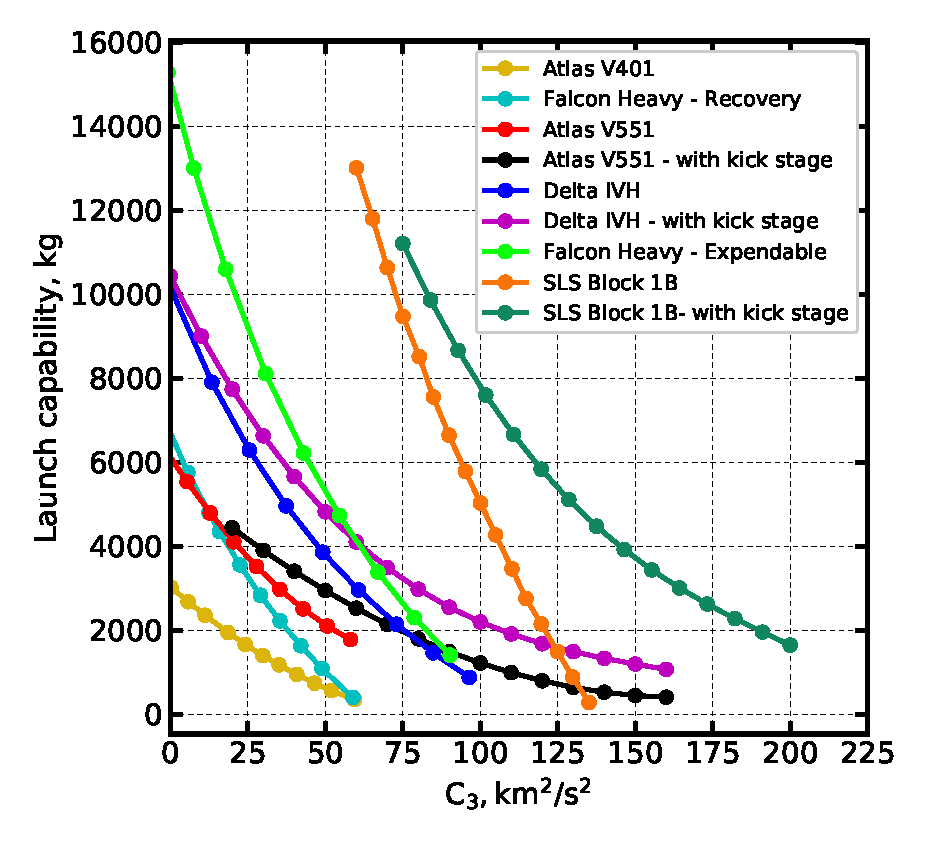
\includegraphics[width=5in]{images/C3-Curves.eps}
\caption{Sample image.}
\label{sample-image}
\end{figure}

\section{Verification and Validation}
\begin{table}[htpb!]
\caption{Sample table title} \label{sample-table}
\begin{center}
\begin{tabular}{|c|c|c|c|c|c|}
  \hline
% after \\: \hline or \cline{col1-col2} \cline{col3-col4} ...
   & $k_{g}$ & $k_{o}$ & $c_{3}$ & $c_{4}$ & $c_{5}$ \\
  \hline\hline
  Careful/Sparse & 0.334 & 0.597 & 1.101 & 9.621 & 8.170 \\ \hline
  Careful/Dense & 3.124 & 3.195 & 1.094 & 5.899 & 7.318 \\ \hline
  Aggressive/Sparse & 0.840 & 9.153 & 2.853 & 8.274 & 0.187 \\ \hline
  Aggressive/Dense & 4.838 & 2.841 & 0.670 & 7.952 & 0.386 \\ \hline
  Hand-Tuned & 0.767 & 0.060 & 0.340 & 2.000 & 0.250 \\
  \hline
\end{tabular}
\end{center}
\end{table}

\section{Sample Test Results with Prototype Tire}

\section{Conclusions}

This is the conclusion.

\subsubsection*{Acknowledgments}
This is the acknowledgement.

\bibliographystyle{apalike}
\bibliography{jfrExampleRefs}

\end{document}